\section{Historia}

El termino \emph{gamification} fue acuñado cerca del año 2008\cite{DefineGamefication}. 
El objetivo fue crear un termino que agrupara todas las ideas y o elementos utilizados en el 
diseño de juegos que pudiesen ser utilizados en otros contextos(distintos a los de entretencion). 
En el año 2010 este termino llega a ser conocido mundialmente que logra aparecer en los \emph{trend} en google\cite{LiCap1.3}, palabras mas buscadas del año.

El concepto basico fue inicialmente utilizado en la decada de los ochenta con el objetivo 
de mejorar y actualizar el juego llamado \emph{MUD}\ref{fig:MudClient}, \emph{Multy User Dungeons}.
El desarrollador,Richard Bartle, comenzo a analizar a los jugadores en donde encontro 4 estereotipos \ref{fig:Players}.

\begin{figure}[!htb]
  \centering
  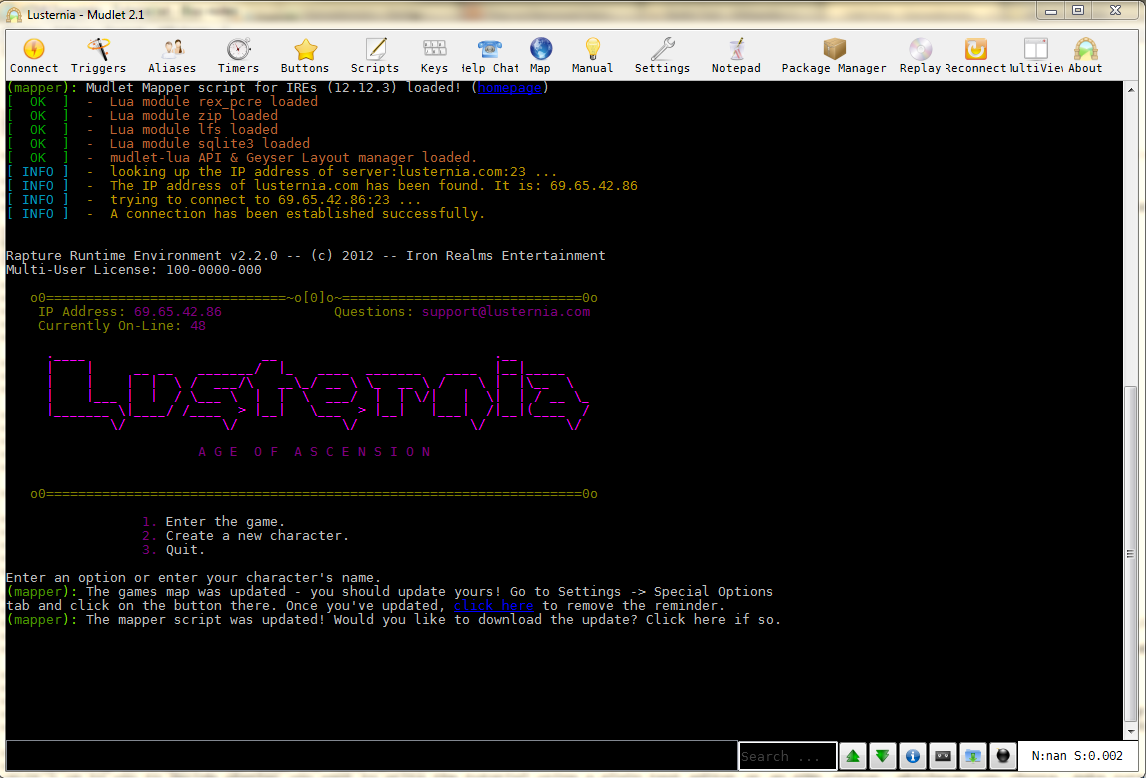
\includegraphics[width=0.5\textwidth]{images/mudclient.png}
  \caption[Caption for LOF]{Real caption\footnotemark}
  \label{fig:MudClient}
\end{figure}

\begin{itemize}

\item \emph{Achievers}: Jugadores que se enfocan en obtener algun exito, obteniendo puntos, premios,
 u otra forma de demostrar el esto. Estos tipos de jugadores se esfuerzan para obtener los premios,
reconocimiento o prestigio, con casi nula ventaja en la jugabilidad o avanze en el juego. Jugadores que
buscan siempre ser los primeros en todo lo posible en un juego obteniendo cada uno de los premios. 

\item \emph{Explorers}: A estos jugadores les gusta explorar el mundo en el cual estan inmerso, mas alla
de lo geografico les interesa encontrar detalles de la jugabilidad. Estos jugadores llegan a conocer
el juego mas que los mismos creadores ya que estudian a fondo todos los aspectos de este. Un
ejemplo de estos son los jugadores solitarios que les gusta descubrir y aventurarse en el mundo.

\item \emph{Killers}: Estos son los mas competitivos. Buscan ser destacados y provocar drama entre usuarios.
Algunos tipos de jugadores que caen en esta categoria son: Trolls, Hacker, Cheaters, entre otroso. Ejemplo 
de este tipo de jugadores son aquellos que se dedican profesionalmente a un juego competitivo.

\item \emph{Socializers}: Personas que sin atraidas por la parte social de los juegos, en desmedro de
la estrategia u otras partes de este. Se puede decir que estos jugadores son el "Corazón" ya que
son los que mas disfrutan con la interaccion entre personas. Para estos, el juego es el vehiculo
que ayuda a crear relaciones entre jugadores. Personas que gustan de jugar en grupos y compartir 
aventuras con jugadores que buscan un objetivo en comun. 

\end{itemize}

Con esta informacion, el desarrollador modifico el juego para satisfacer cada tipo de jugador.
Este cambio tuvo un gran exito y demostro una nueva forma de atraer a diferentes tipos de jugadores a un
juego en particular, esto llamo la atencion de empresas que vieron este concepto como una nueva 
forma de atraer y retener a sus clientes.

\begin{figure}[!htb]
  \centering
  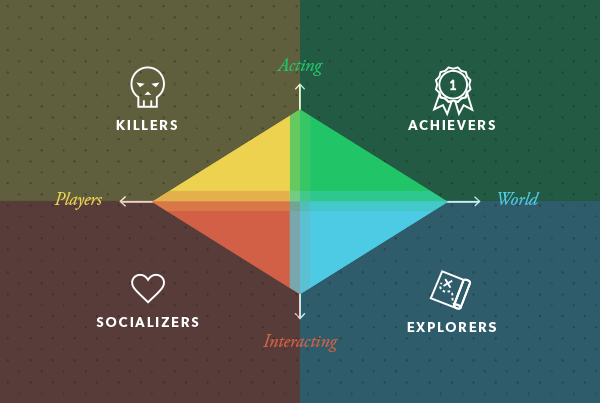
\includegraphics[width=0.5\textwidth]{images/TypeOfPlayersBartle.png}
  \caption[Caption for LOF]{Real caption\footnotemark}
  \label{fig:Players}
\end{figure}

Diversas compañias actualmente usan {\GAM}, varias han creado plataformas para aplicar gamification.
En $2007$, la compañia \emph{Bunchball} \footnote{www.bunchball.com} fue una de las primeras en implementar y proveer
una plataforma gamificada como un servicio\cite{Gam:Bunchball:1}. \emph{Bunchball} tuvo clientes de gran tamaño como
Bravo\footnote{www.bravotv.com} y \emph{The USA network}\footnote{www.usanetwork.com}\cite{Gam:Bunchball:2}.

Otras grandes empresas que utilizan gamificaion en la actualidad son: SAP AG, IBM, EMC, CA, Slalom Consulting,
 Deloitte, Microsoft, LiveOps, RedCritter\cite{Gam:Companies:1}  

Actualmente se han creado eventos dedicados a la discucion acerca el uso de esta tecnica como
\emph{Gamification 2013}, un evento de discucion sobre el futuro de gamification\cite{Gam:Events:1}. 
En $2014$ se llevara a cabo \emph{Loyalty Gamification World Championship} en San Franscico, USA.\cite{Gam:Events:2}

\section{Definicion}

Hoy en dia \emph{gamification} se ha convertido en una herramienta para las empresas 
para poder captar mas clientes. Cada dia aumenta el uso de este concepto por lo que es
necesario entregar una definicion apropiada para el concepto.{\GAM} se puede definir
como el uso de elementos del diseño de juego en contextos diferentes al de entretención. Para entender mejor 
los conceptos bajo esta definicion se explicaran por partes:

\begin{itemize}

\item Juego: En primer lugar este concepto se refiere al juego, en su todo, y no a la accion de jugar.
Este concepto es caracterizado por un conjunto de reglas explicitas que crean un ambiente  
en donde los jugadores buscan la competicion para completar objetivos y metas.

\item Elementos del diseño de juego: Dentro de este concepto se puede encontrar 2 definiciones.
La primera, es una definicion estricta que solo acepta ciertos elementos unicos. La segunda, 
es una definicion en donde todos los elementos pueden ser utilizados. Para llegar a una 
definicion robusta es necesario juntar ambas y asi obtener un conjunto mas restrictivo en donde 
los elementos a utilizar son carateristicos a los juegos, que se encuentran en la mayoria de estos y 
que cumplen una rol importante en la jugabilidad de estos.

\item Contextos diferentes al de juego: Este es el concepto mas complejo de explicar debido a que es una idea  
abstracta. Una forma de explicarla es como una situacion de la vida cotidiana que existe fuera 
de un juego o de un ambiente que contiene \emph{gamification}.

\end{itemize}

\section{Utilizacion}

Esta tecnica a sido utilizada en diferentes areas y contextos en todo el mundo. Marketing ha sido una 
de las areas que ha sido beneficiada con la implementacion de {\GAM}. Mas de 70 empresas en el ranking de 
\emph{Forbes Global $2000$} han utilizado o piensan hacerlo con el motivo de una nueva fuente de 
marketing y como retencion de clientes\cite{Gam:Util:1}. Un ejemplos exitoso del uso en marketing es \emph{Nike} 
con su aplicacion \emph{Nike+ Fuelband} que fue fue lanzada en enero del 2012\cite{Gam:Util:2}. 
Con esta aplicacion se logro crear un sistema gamificado en el cual se ayudaba a sus clientes a manatener 
su forma fisica. Otra empresa multinacional que a utilizado gamification en marketing es \emph{McDonals} 
con el uso de mecanicas de juego derivadas del juego de mesa \emph{Monopoly}. Esta idea viene se viene 
implementando desde $1987$. Gracias a esta idea en el año $2010$ \emph{Mcdonals} incremento sus ventas en los Estados
Unidos en $5.6\%$ \cite{Gam:Util:2}.

\emph{Gamification} tambien es utilizado como una herramienta para atraer y retener clientes,como tambien es
utilizado para alentar el correcto uso de una web. Varias son las empresas que utilizan esta idea, alguna de estas 
son Stack Overflow y Samsung. La primera, web dedicada a preguntas y respuestas sobre tecnologias, entrega puntos
 y o achievements a los usuarios al hacer determinadas tareas. Existen diferentes tipos de medallas y a medida
 de que el usuario va ganando puntos y reputacion va obteniendo privilegios, siendo el mayor de estos 
ayudar a mnoderar el sitio. Samsung por su parte, tambien utiliza puntos y achievements en su web pero
 esta es enfocada a que los usuarios tengan interaccion con la comunidad a nivel de dar reviews de sus 
productos y asi crear contenido para la empresa\cite{Gam:Util:3}. 
Educacion y entrenamiento han sido otras areas en donde a exitido interes por
utilizar \emph{gamification}. En los Estados Unidos el departameto de educacion de la ciudad de neva york
 con el apoyo de \emph{MacArthur Foundation} y \emph{Bill and Melinda Gates Foundation} crearon una escuela
 llamada \emph{Quest to Learn}, Busaqueda para aprender, especializada en el aprendizaje utilizando juegos 
con el objetivo de tranformar la educacion en algo mas atractivo para los niños modernos\cite{Gam:Util:4}. Otro sitio de educcion utilizando esta tecnica 
es \emph{Coursera}, compañia que se apoya de universidades de todo el mundo para enseñar
cursos sobre tecnologias gratis via e-learning. La utilizacion de \emph{gamification}
se ve reflejada en las medallas y certificados dados a medida que el alumno va completando
tareas dentro del curso o completa uno. Dentro de todos los cursos dictados el mas popular es
el de \emph{gamification}\cite{Gam:Util:5}. En el año 2014, se inicio un proyecto llamado
\emph{the True Life Game project} que tiene como objetivo investigar las mejoresformas de
aplicar esta tecnica en la vida cotidiana.

Esta tecnica tambien se usa en mchos otros ambitos, pero en menor cantidad, como produtividad, 
autenticacion, servicios financieros, entre otros.

\section{Criticas}

La idea de \emph{gamification}, desde su despegue, a creado \emph{hype} en todo el mundo ya que ha sido
utilizada por varias compañias, desde micro o pequeñas empresas hasta multinacionales. Pero existen
 retractores a la utilizacion de esta idea en la vida cotidiana. Sebastian Detering, investigador de 
la universidad de Hamburgo, ha dicho que las caracteristicas mas utilizadas no son divertidas y crean 
una sensacion falsa de logro\cite{Gam:Crit:1}.
A esto se a sumado personas relacionadas con el diseño de juegos como son Jon Radoff y Margaret Robertson,
 que declaran que la utilizacion de \emph{gamification} excluye otras partes del diseño
como son la historia, las experiencias de juego y que lo utilizado en este concepto es de lo mas basico 
en donde faltan las mecanicas de juego\cite{Gam:Crit:2}.

En el año 2012, la empresa analista \emph{Gartner} entrego un reporte\cite{Gam:Crit:3} en el cual  
explicaba que la idea de \emph{gamification} "basaba su exito en la nobleza del ususario y del \emph{hype}
de las empresas por utilizar esta idea". Tambien se esperaba de que para el año 2014 el 80$\%$ de las aplicaciones
gamificadas fallarian debido a una falta de buen diseño, esto debido a la falta de seriedad al crear las 
aplicaciones, asi como, el intento de copiar e implementar esto a la mayoria de las ideas.

